\selectlanguage{english}

The Simulation work for this thesis work was carried out using MAT Lab. For this thesis work, we consider the \ac{PL} model that varies uniformly across all the users in the system with the channels drawn from the i.i.d samples. The behavior of the proposed decentralized algorithm is considered for different cell system. The systems convergence behavior and robustness is studied. 

To begin with we consider a \ac{MIMO} model with operating point at 10 dB \ac{SNR}, we consider a system with \me{N_B \, = 2} \ac{BS}s, each equipped with \me{N_T\, = 4} transmit antennas serving \me{k = 3} users each. The allocations for \ac{BS} and users are made by selecting the \ac{BS} with the lowest \ac{PL} component. Fig. 1 (a) shows the  performance of distributed schemes for single antenna recieve system. From the figure a comparission can be made in terms of total rate after each \ac{SCA} update. In figure 1 we can see that all the distributed algorithms converge to the same point

\begin{figure}
	\centering
	\begin{subfigure}[b]{0.75\textwidth}
		\centering
		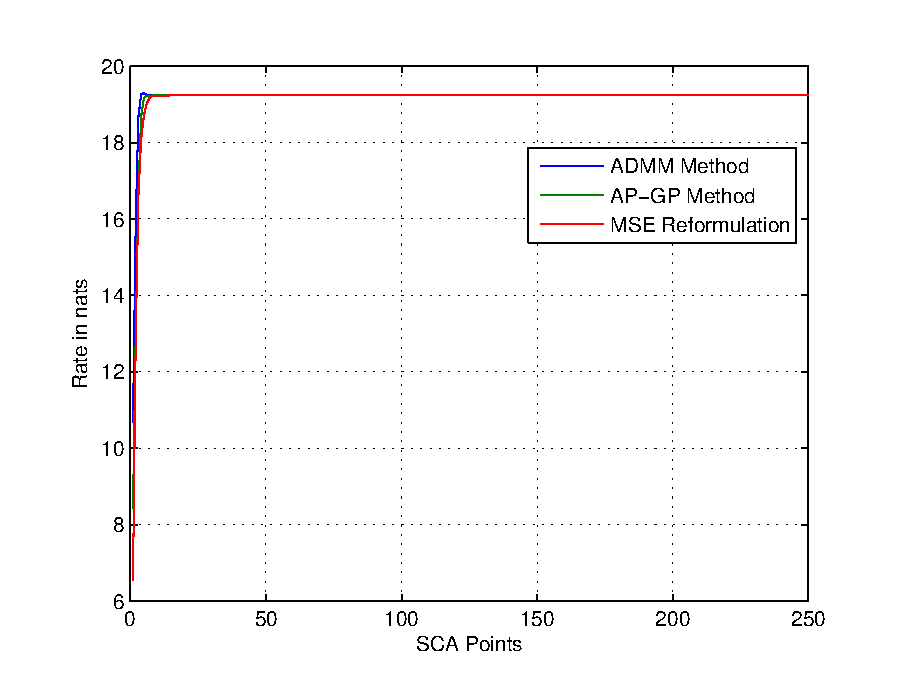
\includegraphics[width=0.75\textwidth]{plot8142}
		\caption{Convergence of sum rate with $N_\mathrm{T} = 8, B = 2, K = 4$, Mobile users}
		\label{fig_1}
	\end{subfigure}
	\begin{subfigure}[b]{0.75\textwidth}
		\centering
		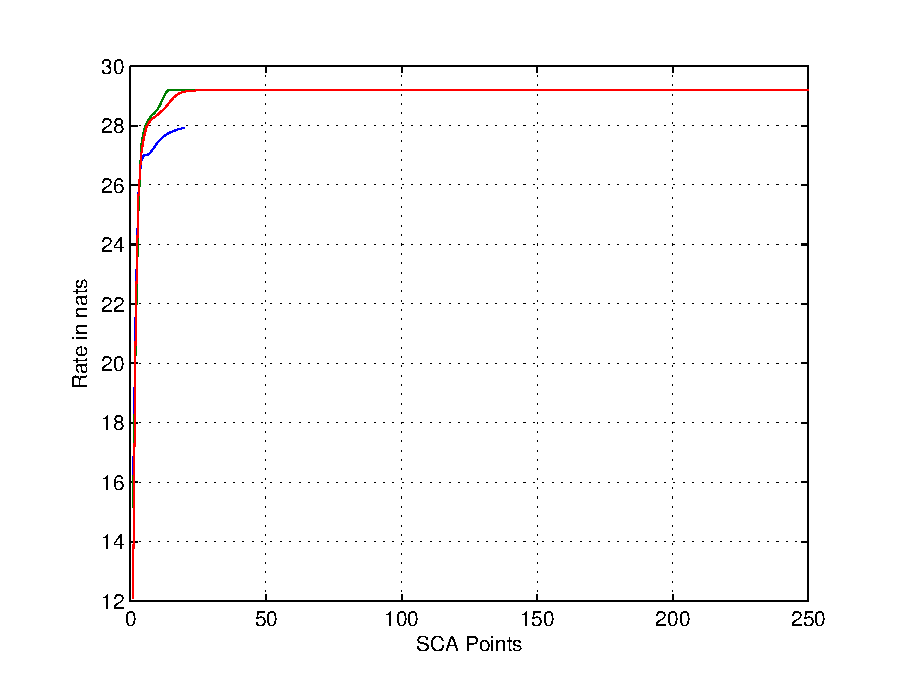
\includegraphics[width=0.75\textwidth]{plot8182}
		\caption{Convergence of sum rate with $N_\mathrm{T} = 8, B = 2, K = 8$, Mobile users}
		\label{fig-2}
	\end{subfigure}
	\caption{Sum rate convergence for mobile users}
	\label{figII}
\end{figure}


\begin{figure}
	\centering
	\begin{subfigure}[b]{0.75\textwidth}
		\centering
		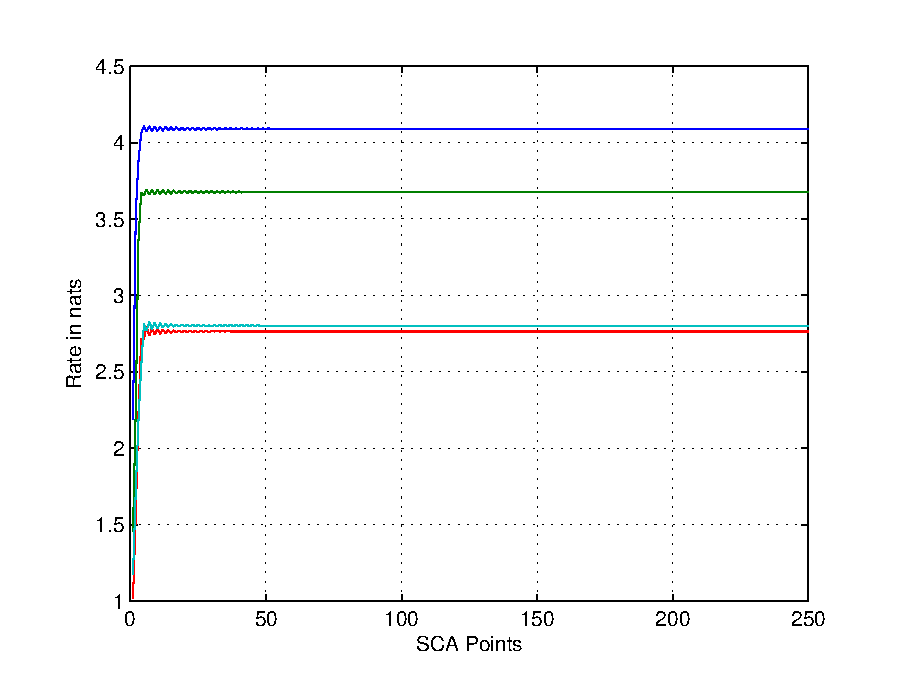
\includegraphics[width=0.75\textwidth]{kktrc8142}
		\caption{Convergence of sum rate with $N_\mathrm{T} = 8, B = 2, K = 4$, Mobile users}
		\label{fig_1}
	\end{subfigure}
	\begin{subfigure}[b]{0.75\textwidth}
		\centering
		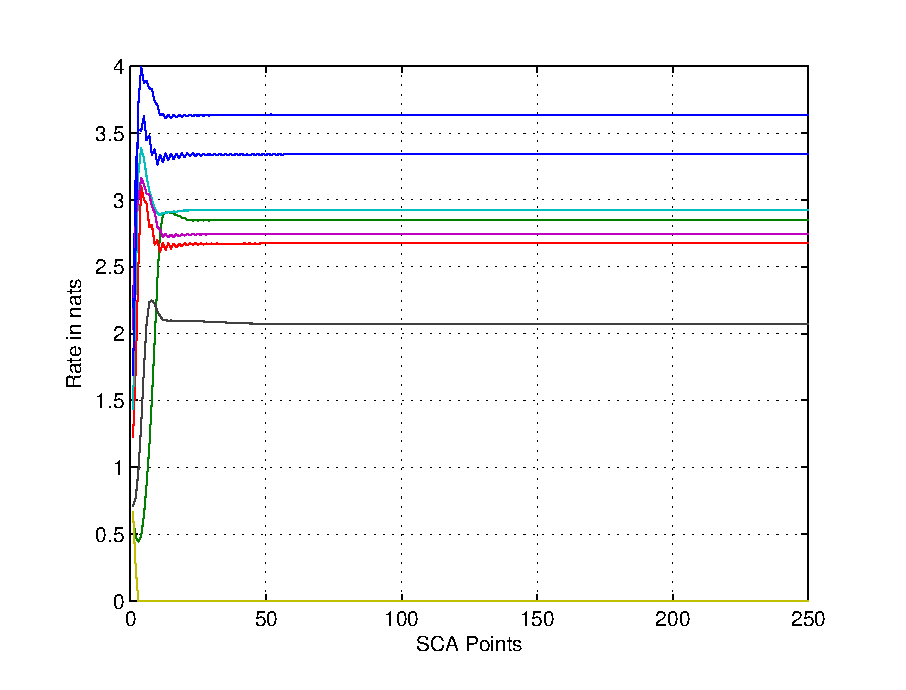
\includegraphics[width=0.75\textwidth]{kkte0rc8182}
		\caption{Convergence of sum rate with $N_\mathrm{T} = 8, B = 2, K = 8$, Mobile users}
		\label{fig-2}
	\end{subfigure}
	\caption{Sum rate convergence for mobile users}
	\label{figII}
\end{figure}

\begin{figure}
	\centering
	\begin{subfigure}[b]{0.75\textwidth}
		\centering
		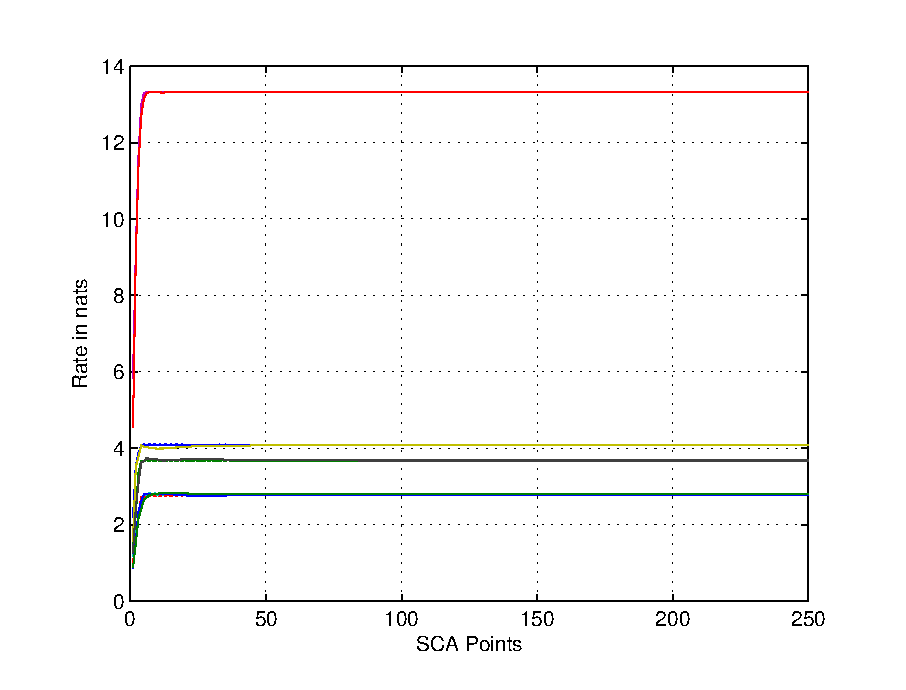
\includegraphics[width=0.75\textwidth]{kktmserc8142}
		\caption{Convergence of sum rate with $N_\mathrm{T} = 8, B = 2, K = 4$, Mobile users}
		\label{fig_1}
	\end{subfigure}
	\begin{subfigure}[b]{0.75\textwidth}
		\centering
		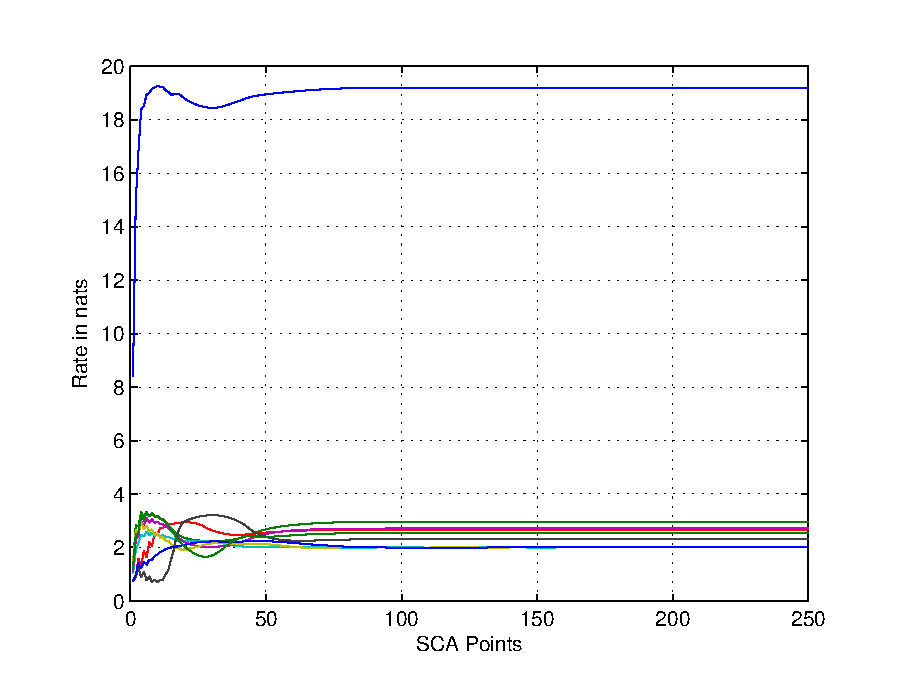
\includegraphics[width=0.75\textwidth]{kktmserc8182}
		\caption{Convergence of sum rate with $N_\mathrm{T} = 8, B = 2, K = $, Mobile users}
		\label{fig-2}
	\end{subfigure}
	\caption{Sum rate convergence for mobile users}
	\label{figIII}
\end{figure}

%\begin{figure}
%\centering
%\begin{subfigure}[b]{0.75\textwidth}
%\centering
%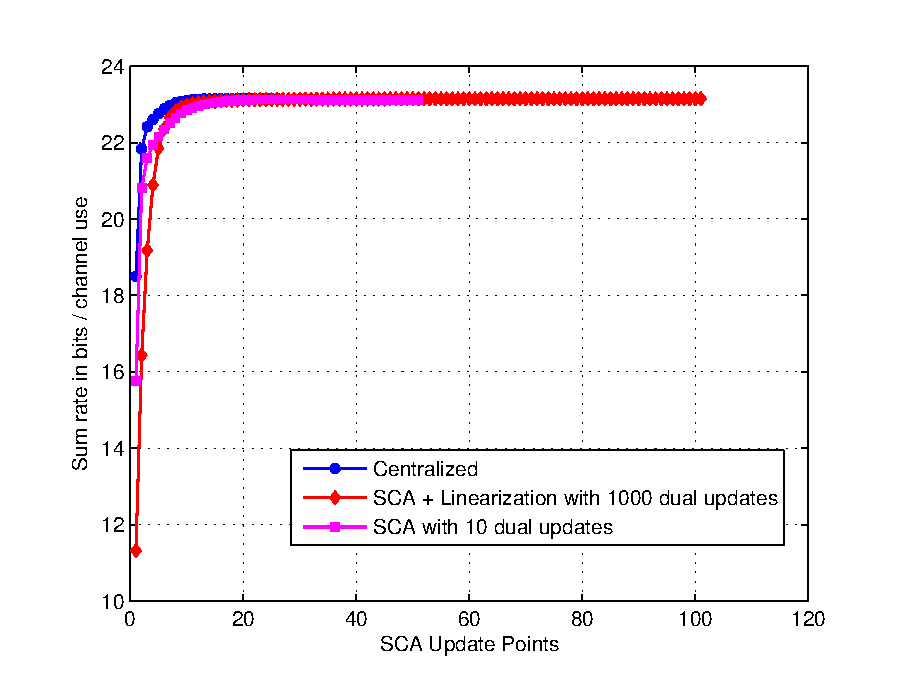
\includegraphics[width=0.75\textwidth]{2_6_8_1}
%\caption{Convergence of sum rate with $N_\mathrm{T} = 8, B = 2, K = 6$, Mobile users}
%\label{fig_1}
%\end{subfigure}
%\begin{subfigure}[b]{0.75\textwidth}
%\centering
%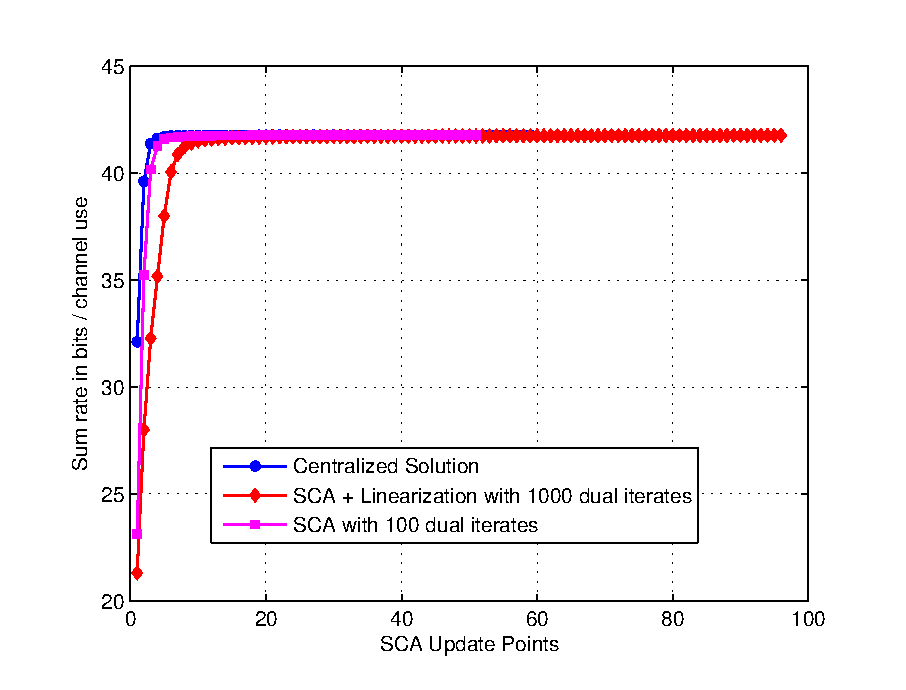
\includegraphics[width=0.75\textwidth]{3_9_12_1}
%\caption{Convergence of sum rate with $N_\mathrm{T} = 12, B = 3, K = 9$, Mobile users}
%\label{fig-2}
%\end{subfigure}
%\caption{Sum rate convergence for mobile users}
%\label{figIV}
%\end{figure}
